\mychapter{Image Processing}{Image Processing}{}
\label{chap:imgpros}

%===========================================================================================================================================================================
\mysection{Introduction}{Introduction}
\label{sec:imgintro}

After modelling the satellite and the auxiliary sensors in Chapter 3, Chapter 4 delves deeper into the theory and methodology used to generate the Earth Tracker measurements.
Firstly, the basic theoretical background of satellite imaging is discussed, including image geometry, different scanning techniques, and typical satellite imagery noise.
This is followed by a discussion of the simplified camera and lens models used in this work, such as the intrinsic and extrinsic camera parameters and common lens distortions.
Finally, the simulator implementation of the Earth Tracker is presented, along with the methodology of how it produces measurements for the pose estimator.

%===========================================================================================================================================================================
\mysection{Satellite Image Characteristics}{Satellite Image Characteristics}
\label{sec:satImgChar}

%===========================================================================================================================================================================
\mysubsection{Imaging Geometry}{Imaging Geometry}
\label{subsec: ImgGeo}

\noindent
All satellite images share a common set of geometric attributes, illustrated in Figure \ref{fig:GSD}. 
The pixel pitch, denoted as $p$, refers to the physical size of a single pixel element on the imaging sensor (for example, one CMOS detector element). 
The sensor width, $s$, represents the total width of the sensor array and is calculated as:
\[
s = I \times p
\]
where $I$ is the number of pixels along one dimension of the image (either horizontally or vertically) typically known as resolution. The swath width, $S_w$, is the total ground area captured by the image and is expressed as:
\[
S_w = I \times GSD
\]
where GSD (Ground Sampling Distance) defines the ground distance represented by each image pixel. Here, $f$ denotes the focal length of the camera, and $h$ the altitude of the satellite. 
The relationship between these parameters can be mathematically expressed as:


\begin{equation}
    \frac{GSD}{p} = \frac{S_w}{s} = \frac{h}{f}
\end{equation}

\begin{figure}[H]
    \centering
    \includegraphics[width=0.4\linewidth]{figures/imageprocessing/GSD.pdf}
    \caption{The relationship between sensor pitch, focal length, satellite altitude, and Ground Sampling Distance (GSD). The pixel pitch ($p$) determines the physical size of each sensor element, while the focal length ($f$) and satellite altitude ($h$) together define how this sensor geometry maps to the ground. A smaller pixel pitch or a longer focal length results in a finer GSD (higher image resolution), whereas increasing altitude enlarges the GSD, reducing spatial resolution.}
    \label{fig:GSD}
\end{figure}

\noindent
The Field of View (FOV) of the satellite is the angle between one image boundary and the opposite image boundary. 
The FOV can be defined in terms of the focal length $f$ and the sensor width $s$ as:

\begin{equation}
    FOV = 2 \, \tan^{-1}\left( \frac{s}{2f} \right)
\end{equation}

\noindent
The FOV can then be used to calculate the swath of the satellite at a specific orbital altitude.
\vspace{0.5cm}

\noindent
GSD is the physical distance between the centers of two adjacent 
pixels measured on the ground in an image captured by the satellite camera.

\noindent
As the $GSD$ depends on the $FOV$, it should be noted that both the $S_w$ and the GSD are affected by the angle 
at which the satellite camera captures the image. This means that the image becomes distorted when taken off-nadir. 
As shown in Figure \ref{fig:OffNadir} in an image by James et al. \cite{OFFN}

\begin{figure}[H]
    \centering
    \includegraphics[width=0.8\linewidth]{figures/imageprocessing/OFFN.png}
    \caption{An illustartion of the distortion of the $GSD$ and $FOV$ of an satellite image when taken Off-Nadir (at an oblique angle) \cite{OFFN}}
    \label{fig:OffNadir}
\end{figure}

\noindent
Figure \ref{fig:OffImg} \cite{EUSI} demonstrates the significant impact an off-nadir angle (ONA) can have on satellite imagery. While ONA is often discussed in 
relation to its effect on ground sample distance (GSD), the implications extend well beyond image resolution. Viewing the Earth from an angle alters the scene's geometry, 
introducing distortions that can shift feature positions and complicate image interpretation. These effects become particularly challenging when integrating imagery 
with Digital Elevation Maps (DEMs), which are typically referenced to a nadir viewing geometry. Applying such DEMs to high-ONA imagery can result in inaccurate 
terrain corrections, feature misalignment, and increased geolocation errors. In regions with substantial elevation variation, these issues are amplified, reducing 
the accuracy of orthorectification and making reliable feature extraction more difficult.


\begin{figure}[H]
    \centering
    \begin{subfigure}[b]{0.48\linewidth}
        \centering
        \includegraphics[width=\linewidth]{figures/imageprocessing/6ONA.png}
        \caption{The Eiffel tower taken with a 6 Degree off-nadir angle.}
        \label{fig:ONA1}
    \end{subfigure}
    \hfill
    \begin{subfigure}[b]{0.48\linewidth}
        \centering
        \includegraphics[width=\linewidth]{figures/imageprocessing/44ONA.png} % <-- Replace with your actual image path
        \caption{The Eiffel tower taken with a 44 degree off-nadir angle.}
        \label{fig:ONA2}
    \end{subfigure}
    \caption{The effect off-nadir angle on satellite imagery.}
    \label{fig:OffImg}
\end{figure}


%==============================================================================================================================================================================
\mysubsection{Image Resolution}{Image Resolution}

Satellite imagery is a fundamental tool for observing and monitoring the Earth's surface. The quality and usefulness of these images are determined by several key characteristics, including spatial, temporal, radiometric, and spectral resolution. Each of these parameters influences the level of detail, frequency of observation, and type of information that can be extracted from the imagery. In this section, we provide an overview of these properties and illustrate their effects with representative examples.

%======================================================================================================================================================================

\mysubsubsection{Spatial Resolution}{Spatial Resolution}
\noindent
\noindent
As defined in \ref{sec:satImgChar} the GSD defines the spatial resolution of a satellite image, indicating the level of detail that can be resolved on the ground. Smaller GSD values correspond to higher resolution, enabling finer features to be distinguished. This is illustrated in Figure \ref{fig:GSD_all}, where a GSD of 40 m results in lower resolution compared to a GSD of 10 m.


\begin{figure}[H]
    \centering
    \begin{subfigure}[b]{0.32\linewidth}
        \centering
        \includegraphics[width=\linewidth]{figures/imageprocessing/10.png}
        \caption{GSD of 10m}
        \label{fig:GSD1}
    \end{subfigure}
    \hfill
    \begin{subfigure}[b]{0.32\linewidth}
        \centering
        \includegraphics[width=\linewidth]{figures/imageprocessing/20.png}
        \caption{GSD of 20m}
        \label{fig:GSD2}
    \end{subfigure}
    \hfill
    \begin{subfigure}[b]{0.32\linewidth}
        \centering
        \includegraphics[width=\linewidth]{figures/imageprocessing/40.png}
        \caption{GSD of 40m}
        \label{fig:GSD3}
    \end{subfigure}
    \caption{Illustration of the relationship between spatial resolution and Ground Sampling Distance (GSD). As GSD increases, each pixel represents a larger area on the ground, resulting in lower image resolution and less detail. Conversely, smaller GSD values correspond to higher resolution, capturing finer features in the scene.}
    \label{fig:GSD_all}
\end{figure}

\mysubsubsection{Temporal Resolution}{Temporal Resolution}
\noindent
Just as satellites have spatial resolution, they also have temporal resolution. Temporal resolution is defined by the frequency with which a satellite 
revisits a site or target area. For example, Sentinel-2A and Sentinel-2B have a revisit rate of 10 days individually \cite{Wang}, 
resulting in a temporal resolution of 5 days. This means that by increasing the number of satellites in a constellation, a higher temporal resolution can be 
achieved. An example of a tree growing is illustrated in Figure \ref{fig:TempRes} \cite{Tree}, showing that the higher temporal resolution implies that an area could be observed to be growing steadily and conversily the lower the temporal resolution the more rapid the growth of a area might be seen, indicating less temporal detail. Many satellites with high temporal resolution are placed in sun-synchronous orbits, which are near-polar and allow the satellite to pass over the same location at approximately the same local solar time each day.

\begin{figure}[H]
    \centering
    \includegraphics[width=\linewidth]{figures/imageprocessing/Temporal Resolution.png}
    \caption{Illustration of temporal resolution in satellite imagery represented by a tree growing \cite{Tree}. Temporal resolution refers to how frequently a satellite revisits the same location. Higher temporal resolution, achieved by shorter revisit intervals or larger satellite constellations, allows changes on the ground, such as vegetation growth or urban development, to be monitored more closely over time.}
    \label{fig:TempRes}
\end{figure}

\mysubsubsection{Radiometric resolution}{Radiometric resolution}
\noindent
A satellite imager also has two other important characteristics: radiometric resolution and spectral resolution. 
Radiometric resolution describes the sensor's ability to detect small differences in energy and is usually expressed in bits. 
For instance, an 8-bit sensor can record 256 levels of intensity, while a 12-bit sensor can capture 4096 levels. 
Spectral resolution, by contrast, refers to the sensor's ability to distinguish between different wavelengths of light. 
Since sunlight contains a broad range of wavelengths, multispectral imagers (MSI) are designed to respond to specific bands or groups of wavelengths. 
These may include visible bands such as red, green, and blue, as well as near-infrared (NIR) and shortwave infrared (SWIR). 
Some sensors, such as panchromatic imagers, cover a wide wavelength range and produce high-resolution black-and-white images. 
Multispectral and hyperspectral systems are widely used for vegetation monitoring (such as the use of normalized difference vegetation index), water quality studies, mineral exploration, and land-use mapping. 
Because each material reflects and absorbs light differently across the electromagnetic spectrum, these sensors make it possible to identify and track environmental changes over time. 
An example is shown in Figure~\ref{fig:MSI}, which illustrates the spectral bands typically used by a multispectral imager.


\begin{figure}[H]
    \centering
    \begin{subfigure}[b]{0.32\linewidth}
        \centering
        \includegraphics[width=\linewidth]{figures/imageprocessing/FalseColour.png}
        \caption{False Colour (NIR)}
        \label{fig:FalseColour}
    \end{subfigure}
    \hfill
    \begin{subfigure}[b]{0.32\linewidth}
        \centering
        \includegraphics[width=\linewidth]{figures/imageprocessing/NDVI.png}
        \caption{Normalised Difference Vegetation Index (NDVI)}
        \label{fig:NDVI}
    \end{subfigure}
    \hfill
    \begin{subfigure}[b]{0.32\linewidth}
        \centering
        \includegraphics[width=\linewidth]{figures/imageprocessing/SWIR.png}
        \caption{Short-Wave Infrared (SWIR)}
        \label{fig:SWIR}
    \end{subfigure}
    \caption{Images are captured using different wave lengths and reconstructed to convey different information.}
    \label{fig:MSI}
\end{figure}

%==============================================================================================================================================================
\mysubsection{Image Detectors}{Image Detectors}

Most Earth observation satellites can be categorized into three types of sensors: pushbroom, whiskbroom, and snapshot \cite{Fowler,Nag}. Without going into too 
much detail, the basic concepts of each sensor mechanism are illustrated in Figure \ref{fig:Detectors}. A background image is used to convey the concept, although 
in reality, each sensor element captures just one pixel at a time. The pushbroom sensor, shown in Figure \ref{fig:Pushbroom}, is a type of imager that captures one row of pixels at a time. It relies on the satellite's 
forward motion to build up the second dimension of the image over time. The whiskbroom sensor, illustrated in Figure \ref{fig:Whiskbroom}, captures one pixel at a time by scanning from one side of the swath to the other using a 
rotating mirror. Like the pushbroom sensor, it also depends on the satellite's movement to form a complete image. Finally, the snapshot sensor, shown in Figure \ref{fig:Snapshot}, captures a 2D array of the scene in a single time step. Snapshot sensors are considered to 
have a global shutter, as the entire image is acquired simultaneously.

\begin{figure}[H]
    \centering
    % First row: Pushbroom and Whiskbroom
    \begin{subfigure}[b]{0.45\linewidth}
        \centering
        \includegraphics[width=\linewidth]{figures/imageprocessing/CameraSensor1.pdf}
        \caption{Pushbroom}
        \label{fig:Pushbroom}
    \end{subfigure}
    \hfill
    \begin{subfigure}[b]{0.45\linewidth}
        \centering
        \includegraphics[width=\linewidth]{figures/imageprocessing/CameraSensor2.pdf}
        \caption{Whiskbroom}
        \label{fig:Whiskbroom}
    \end{subfigure}

    \par\bigskip % Adds vertical spacing and starts a new line

    % Second row: Snapshot Camera centered
    \begin{subfigure}[b]{0.4\linewidth}
        \centering
        \includegraphics[width=\linewidth]{figures/imageprocessing/CameraSensor3.pdf}
        \caption{Snapshot Camera}
        \label{fig:Snapshot}
    \end{subfigure}

    \caption{Images are captured using different imager detectors.}
    \label{fig:Detectors}
\end{figure}

%======================================================================================================================================================================
\mysubsection{Environmental Noise}{Environemental Noise}

Several types of noise and environmental factors can impact the quality and usability of satellite imagery. Among the most significant are 
atmospheric interference, cloud cover, and variations due to the time of day or season.
\vspace{0.5cm}

\noindent
Atmospheric effects play a major role in distorting satellite images. As light from the Earth's surface travels through the 
atmosphere to reach the satellite sensor, it is subject to scattering and absorption. Particles such as dust, water vapor, and aerosols can 
scatter incoming light, particularly in shorter wavelengths (e.g., blue), which leads to hazing and reduced image contrast. Atmospheric correction 
algorithms are often applied during post-processing to compensate for these effects, as we can see in Figure \ref{fig:Atmos} \cite{Atmos, Dove}
\vspace{0.5cm}

\begin{figure}[H]
    \centering
    \includegraphics[width=\linewidth]{figures/imageprocessing/scattering.png}
    \caption{Difference in satellite imagery due to atmospheric asoption and scattering \cite{Atmos, Dove}}
    \label{fig:Atmos}
\end{figure}

\noindent
Cloud cover is another major challenge for optical imaging systems. Thick clouds can block the land surface entirely, making it impossible to capture useful data in 
those areas. Even thin clouds or their shadows can change the spectral signature of a scene, which makes interpretation and classification less reliable. To deal with this, 
cloud detection and masking methods are often applied, and satellites with higher temporal resolution are used so that cloud-free images can be captured at a later time.

\vspace{0.5cm}

\begin{figure}[H]
    \centering
    \begin{subfigure}[b]{0.48\linewidth}
        \centering
        \includegraphics[width=\linewidth]{figures/imageprocessing/Cape1.jpg}
        \caption{Cape Town without cloud cover.}
        \label{fig:Cloud1}
    \end{subfigure}
    \hfill
    \begin{subfigure}[b]{0.48\linewidth}
        \centering
        \includegraphics[width=\linewidth]{figures/imageprocessing/Cape2.jpg} % <-- Replace with your actual image path
        \caption{Cape Town with cloud cover.}
        \label{fig:Cloud2}
    \end{subfigure}
    \caption{The effect of cloud cover changing the spectral signature of and image.}
    \label{fig:Cloud}
\end{figure}

\noindent
Time of day and time of year also have a substantial influence on image appearance and quality. Images captured at different times of the day may 
exhibit differences in shadow length and direction, which can affect the visual interpretation or performance of automated analysis algorithms. Seasonal changes 
can also drastically alter the landscape, with vegetation, snow cover, and water bodies all exhibiting different spectral signatures depending on the time of year. For example, 
a forest may appear lush and green in summer but sparse and brown in winter, even though the physical structure of the landscape remains unchanged.
\vspace{0.5cm}

\begin{figure}[H]
    \centering
    \begin{subfigure}[b]{0.48\linewidth}
        \centering
        \includegraphics[width=\linewidth]{figures/imageprocessing/Cape1.jpg}
        \caption{Cape Town in the wet season.}
        \label{fig:Time1}
    \end{subfigure}
    \hfill
    \begin{subfigure}[b]{0.48\linewidth}
        \centering
        \includegraphics[width=\linewidth]{figures/imageprocessing/Cape3.jpg}
        \caption{Cape Town in the dry season.}
        \label{fig:Time2}
    \end{subfigure}
    \caption{The effect of seasonal and time differences.}
    \label{fig:Time}
\end{figure}

\noindent
Therefore, when analyzing or comparing satellite images, it is essential to consider these factors to ensure accurate interpretation and to 
avoid drawing incorrect conclusions from noisy or inconsistent data.

%===============================================================================================================================================================
\mysection{Camera Model}{Camera Model}

Accurate modeling of a satellite camera is essential for understanding how three-dimensional scenes are projected onto a two-dimensional image plane. 
The camera model defines the geometric and photometric relationships between points in the observed scene and their corresponding image measurements. 
This section introduces the fundamental concepts of camera modeling, beginning with the idealized pinhole model, followed by the definition of intrinsic parameters that map the camera's projection onto a pixel-based image, and finally the extrinsic parameters that relate the camera frame to the satellite body frame. 
Together, these models form the basis for projecting and interpreting satellite imagery in subsequent image processing and state estimation tasks.

%================================================================================================================================================================
\mysubsection{Pinhole Model}{Pinhole Model}

\noindent
The ideal pinhole camera model can be represented as a geometric configuration consisting of an image plane and an optical center, also referred to as the pinhole. 
Light rays originating from a point in the observed scene pass through the optical center and intersect the image plane, forming an inverted image of the object. 
The distance between the optical center and the image plane is defined as the focal length, denoted by $f$, as illustrated in Figure \ref{fig:pinhole}. 

\begin{figure}[H]
    \centering
    \includegraphics[width=1\linewidth]{figures/imageprocessing/PinholeModel3.pdf}
    \caption{A satellite imager illustrated as an ideal pinhole model camera.}
    \label{fig:pinhole}
\end{figure}

\noindent
The projection from the three-dimensional camera coordinate system $\mathcal{C}$ to the two-dimensional image plane $\mathcal{M}$ is governed by the pinhole camera equation:

\begin{equation}
\begin{bmatrix}
    x_\mathcal{M} \\
    y_\mathcal{M} \\
    -f
\end{bmatrix}
= \frac{-f}{z_\mathcal{C}}
\begin{bmatrix}
    x_\mathcal{C} \\
    y_\mathcal{C} \\
    z_\mathcal{C}
\end{bmatrix}
\end{equation}

\noindent
As illustrated in Figure \ref{fig:pinhole}, this projection inherently produces an inverted image, where the $x$ and $y$ axes are flipped with respect to the original scene.
\vspace{0.5cm}

\noindent
To fit into our transformation scheme this work has established in Chapter 3. This equation can be rewritten as a transformation matrix

\begin{equation}
    \mathbf{T}_\mathcal{C}^\mathcal{M} = 
    \begin{bmatrix}
        \frac{-f}{z_\mathcal{C}}    & 0                             & 0                          & 0 \\
        0                           & \frac{-f}{z_\mathcal{C}}      & 0                          & 0 \\
        0                           & 0                             & \frac{-f}{z_\mathcal{C}}   & 0 \\
        0                           & 0                             & 0                          & 1        
    \end{bmatrix}
    \text{.}
\end{equation}

%=====================================================================================================================================================================
\mysubsection{Intrinsic Camera Matrix}{Intrinsic Camera Matrix}

In digital image representation, the $\bar{x}_\mathcal{P}$-axis typically increases from left to right, and the $\bar{y}_\mathcal{P}$-axis increases from top to bottom, which differs from
the conventional mathematical representation of the image plane as can be seen in Figure \ref{fig:PixelPlane}. Consequently, an additional transformation is required to map the projected coordinates to the pixel 
coordinate system. Thus the projection plane coordinates of the projected feature point $\mathbf{f}_\mathcal{M}$ can be converted into pixel based measurements by creating a projection matrix also known as
the intrinsic camera matrix.

\begin{figure}[H]
    \centering
    \includegraphics[width=0.4\linewidth]{figures/imageprocessing/ImagePlane1.pdf}
    \caption{The realtionship between the camera refernce frame and the pixel plane reference frame.}
    \label{fig:PixelPlane}
\end{figure}

\noindent
Firstly, a horizontal and verticle scale factor $s_x$ and $s_y$ need to be defined as 

\begin{equation}
    s_x = \frac{I_x}{SensorWidth}
    \text{, and}
\end{equation}

\begin{equation}
    s_x = \frac{I_y}{SensorHeight}
    \text{.}
\end{equation}

\noindent 
In the above equations, image resolution $I_x$ and $I_y$ refers to the size, in pixels, of the resulting image captures by the modelled camera. $SensorWidth$ and $SensorHeight$ refers to the physical
size of the sensor array, this means the scaling factors $s_x$ and $s_y$ can be seen as having a unit of pixels per distance. This can also be interpreted as the reciprocal of pitch 
$p$ which is defined as distance per pixel.
\vspace{0.5cm}

\noindent
Pixel based coordinates of the projected point in this case a feature point $[x_\mathcal{M}, y_\mathcal{M},1]$ can be calculated with,

\begin{equation}
    \begin{bmatrix}
    x_\mathcal{P} \\
    y_\mathcal{P} \\
    1    
    \end{bmatrix}
    =
    \begin{bmatrix}
        s_x & 0  & 0 \\
        0 & -s_y & 0 \\
        0 & 0 & 1
    \end{bmatrix}
    \begin{bmatrix}
        x_\mathcal{M} \\ 
        y_\mathcal{M} \\
        1
    \end{bmatrix}
    \label{Eq:PM}
\end{equation}

\noindent 
Note the negative sign infront of $s_y$ as the y-axis are flipped as seen in Figure \ref{fig:PixelPlane}. The intrinsic matrix in 
Equation \ref{Eq:PM} can lastly be expanded with the offsets $c_x$ amd $c_y$ that ensure that the pixel-based projection plane coordinates are in the lower-right 
quadrant, as in the convention with digital image. These offsets are defined as:

\begin{equation}
    c_x = \frac{I_x}{2} \text{, and}
\end{equation}

\begin{equation}
    c_y = \frac{I_y}{2} \text{.}
\end{equation}

\noindent
Pixel-based coordinated off the projected point $[x_\mathcal{M}, y_\mathcal{M},1]^T$ can be calculated in the typical convention with

\begin{equation}
\begin{split}
    \begin{bmatrix}
        x_\mathcal{P} \\
        y_\mathcal{P} \\
        1
    \end{bmatrix}
    &=
    \begin{bmatrix}
        s_x & \alpha & c_x \\
        0 & -s_y    & c_y \\
        0 & 0 & 1
    \end{bmatrix}
    \begin{bmatrix}
        x_\mathcal{M} \\
        y_\mathcal{M} \\
        1
    \end{bmatrix} \\[6pt]
    &=
    \mathbf{K}
    \begin{bmatrix}
        x_\mathcal{M} \\
        y_\mathcal{M} \\
        1
    \end{bmatrix}
\end{split}
\end{equation}

\noindent
where $\mathbf{K}$ is known as the intrinsic matrix. A skewing factor of $\alpha$ is added to adjust for skewing effects of the camera.
\vspace{0.5cm}

\noindent 
The tranditional $\mathbf{K}$ matrix can be manipluated to look like our previously defined transformation matrixes, where the z-axis is added to keep the vector format.

\begin{equation}
    \mathbf{T}_\mathcal{C}^\mathcal{P} = 
    \begin{bmatrix}
        s_x     & \alpha        & 0  & c_x  \\
        0       & -s_y          & 0  & c_y  \\
        0       & 0             & 1 & 0    \\
        0       & 0             & 0  & 1        
    \end{bmatrix}
\end{equation}



%====================================================================================================================================================================
\mysubsection{Extrinsic Camera Matrix}{Extrinsic Camera Matrix}

\noindent
In the projection equations, it is typically assumed that the point being projected onto the image plane is already expressed in the camera reference frame. 
However, this is not always the case. In certain situations, the points to be projected must first be transformed into the camera reference frame. 
\vspace{0.5cm}

\noindent
We need to relate the extrinsic camera frame to the body reference frame and the corresponding DCM is defined as:

\begin{equation}
    \mathbf{A}_\mathcal{B}^\mathcal{C} =
    \begin{bmatrix}
        -1 & 0 & 0\\
         0 & -1 & 0\\
         0 & 0 & 1
    \end{bmatrix}
\end{equation}

\noindent
It is assumed that the origins of the body frame $\mathcal{B}$ and the camera reference frame $\mathcal{C}$ coincide, so no translation is required. Thus the transformation matrix can be
expressed as:

\begin{equation}
    \mathbf{T}_\mathcal{B}^\mathcal{C} = 
    \begin{bmatrix}
        \mathbf{A}_\mathcal{B}^\mathcal{C} & \boldsymbol{0}_{3\times1} \\
        \boldsymbol{0}_{1\times3} & 1
    \end{bmatrix}
\end{equation}

\noindent
Thus, the complete transformation chain for converting a 3D feature vector in the body frame to a feature pixel in the pixel plane is:
\begin{equation}
    \mathbf{f}_\mathcal{P}^+ = 
    \mathbf{T}_\mathcal{M}^\mathcal{P} \times
    \mathbf{T}_\mathcal{C}^\mathcal{M} \times  
    \mathbf{T}_\mathcal{B}^\mathcal{C} \times 
    \mathbf{f}_\mathcal{B}^+
\end{equation}


%========================================================================================================================================================================
\mysection{Lens Distortion}{Lens Distortion}

\noindent
There are many types of lens distortions that can affect satellite imagery. In this work, we focus on the two primary geometric distortions: radial distortion and tangential distortion \cite{Wang}. 
Additionally, chromatic aberration will be addressed, although other distortions exist beyond the scope of this study. 
As background for modeling these distortions, the following equation defines the squared distance of a pixel from the lens center:

\begin{equation}
    r^2 = \mathbf{x}_{\mathcal{P},n}^2 + \mathbf{y}_{\mathcal{P},n}^2
    \label{eq:radialDistance}
\end{equation}

\noindent
Here, $\mathbf{x}_{\mathcal{P},n}$ and $\mathbf{y}_{\mathcal{P},n}$ represent the undistorted pixel coordinates, and $r$ is the radial distance from the optical center of the lens.

%=======================================================================================================================================================================
\mysubsection{Radial Distortion}{Radial Distortion}

Radial distortion, also referred to as barrel or pincushion distortion, is a type of lens aberration in which straight lines appear increasingly curved as their 
distance from the optical centre grows as seen in Figure \ref{fig:RadialDisortion}. This effect is caused by imperfections in the lens geometry, leading to magnification that varies with radial distance 
from the image centre. Barrel distortion causes lines to bow outward, while pincushion distortion causes them to bend inward, each altering the perceived 
shape of objects in the image. This distortion is goverend by

\begin{equation}
    \begin{split}
    \mathbf{x}_{\mathcal{P},r}  &= \mathbf{x}_{\mathcal{P},n}(1 + k_1r^2 + k_2r^4 + k_3r^6) \\
    \mathbf{y}_{\mathcal{P},r}  &= \mathbf{y}_{\mathcal{P},n}(1+ k_1r^2 + k_2r^4 + k_3r^6)
    \end{split}
\end{equation}

\noindent
Here, $\mathbf{x}_{\mathcal{P},r}$ and $\mathbf{y}_{\mathcal{P},r}$ are the radially distorted pixel coordinates, while $\mathbf{x}_{\mathcal{P},n}$ and $\mathbf{y}_{\mathcal{P},n}$ are the original, undistorted pixels. 
The variable $r$ is the radial distance from the optical center, defined in Equation \ref{eq:radialDistance}. 
The coefficients $k_1$, $k_2$, and $k_3$ control the magnitude and shape of the distortion, with higher-order terms affecting distortion further from the center.

\begin{figure}[H]
    \centering
    \begin{subfigure}[b]{0.48\linewidth}
        \centering
        \includegraphics[width=\linewidth]{figures/imageprocessing/10.png}
        \caption{Image without radial distortion}
        \label{fig:RD1}
    \end{subfigure}
    \hfill
    \begin{subfigure}[b]{0.48\linewidth}
        \centering
        \includegraphics[width=\linewidth]{figures/imageprocessing/RadialDistortion.jpg}
        \caption{Image with radial distortion}
        \label{fig:Radial2}
    \end{subfigure}
    \caption{Radial lens disortion applied to an satellite image of Cape Town stadium.}
    \label{fig:RadialDisortion}
\end{figure}

%=======================================================================================================================================================================
\mysubsection{Tangential Distortion}{Tangential Distortion}

Tangential distortion is a type of lens distortion in which the image appears as if it has been tilted or skewed, making it look misaligned with the 
sensor array as ween in Figure \ref{fig:TangentialDisortion}. This effect occurs when the lens and image sensor are not perfectly parallel, causing light rays to intersect the sensor at an angle. As a 
result, straight lines may appear slanted, and the overall image geometry can be subtly warped.

\begin{equation}
    \begin{split}
    \mathbf{x}_{\mathcal{P},t}  &= 2p_1\mathbf{x}_{\mathcal{P},n} \mathbf{y}_{\mathcal{P},n}  + p_2(r^2 + 2\mathbf{x}_{\mathcal{P},n} ^2) \\
    \mathbf{y}_{\mathcal{P},t}  &= p_1(r^2 + 2\mathbf{y}_{\mathcal{P},n} ^2) + 2p_2\mathbf{x}_{\mathcal{P},n} \mathbf{y}_{\mathcal{P},n}
    \end{split}
\end{equation}

\noindent
Here, $\mathbf{x}_{\mathcal{P},t}$ and $\mathbf{y}_{\mathcal{P},t}$ are the tangentially distorted pixel coordinates, while $\mathbf{x}_{\mathcal{P},n}$ and $\mathbf{y}_{\mathcal{P},n}$ are the original, undistorted pixels. 
The variable $r$ is the radial distance from the optical center, as defined in Equation \ref{eq:radialDistance}. 
The coefficients $p_1$ and $p_2$ represent the tangential distortion parameters, controlling the degree of image skew caused by misalignment between the lens and sensor. 
Higher values of these coefficients result in greater apparent tilting or warping of the image.


\begin{figure}[H]
    \centering
    \begin{subfigure}[b]{0.48\linewidth}
        \centering
        \includegraphics[width=\linewidth]{figures/imageprocessing/10.png}
        \caption{Image without tangential distortion}
        \label{fig:TD1}
    \end{subfigure}
    \hfill
    \begin{subfigure}[b]{0.48\linewidth}
        \centering
        \includegraphics[width=\linewidth]{figures/imageprocessing/TangentialDistortion.png}
        \caption{Image with tangential distortion}
        \label{fig:TD2}
    \end{subfigure}
    \caption{Tangential lens disortion applied to a satellite image of Cape Town stadium.}
    \label{fig:TangentialDisortion}
\end{figure}

%=======================================================================================================================================================================

\noindent
The total geometric distortion can be expressed as the sum of the radial distortion and the tangential distortion components as shown in Equation \ref{Eq:Distortion}. Together, these
distortions describe how the lens alters the true geometry of the scene, affecting both the curvature and alignment of image features. Accurate modelling and correction of both 
components are essential in satellite camera calibration, where precise spatial measurements are required.

\begin{equation}
    \begin{split}
    \mathbf{x}_{\mathcal{P},d} = \mathbf{x}_{\mathcal{P},r}  + \mathbf{x}_{\mathcal{P},t}  \\
    \mathbf{y}_{\mathcal{P},d}  = \mathbf{y}_{\mathcal{P},r}  + \mathbf{y}_{\mathcal{P},t}  \\        
    \end{split}
    \label{Eq:Distortion}
\end{equation}

%====================================================================================================================================================================
\mysubsection{Chromatic Abberation}{Chromatic Abberation}

Chromatic aberration arises from the nature of light itself. White light is a combination of many wavelengths. Since lenses use refraction to focus light rays, 
different wavelengths bend by different amounts. As a result, red light will focus on a different plane than green, which in turn focuses on a different plane 
than blue. Blue light is refracted the most, causing an enlarging effect, as its focal point is closest to the lens as illustrated in Figure \ref{fig:Chroma}. The Figure \ref{fig:CA} shows the effect of chormatic abberation in the lens, with the effect most promanant on the edges of the image.
\vspace{0.5cm}

\begin{figure}[H]
    \centering
    \includegraphics[width=0.8\linewidth]{figures/imageprocessing/Chromatic_aberration.pdf}
    \caption{The effect of the lens on different wave lengths of light which will cause some wavelenghts to be out of focus and enlarged. \cite{Chroma}}
    \label{fig:Chroma}
\end{figure}

\noindent
This is done by separating the image into its red, green, and blue channels, enlarging each channel by a different scale factor, and then 
recombining them into a single RGB image. As a result, the blue channel appears the largest, followed by the green channel, with the red channel appearing smallest.

\begin{figure}[H]
    \centering
    \begin{subfigure}[b]{0.48\linewidth}
        \centering
        \includegraphics[width=\linewidth]{figures/imageprocessing/10.png}
        \caption{Original Image}
        \label{fig:CA1}
    \end{subfigure}
    \hfill
    \begin{subfigure}[b]{0.48\linewidth}
        \centering
        \includegraphics[width=\linewidth]{figures/imageprocessing/10_chromatic.png}
        \caption{Image with chromatic abberation}
        \label{fig:CA2}
    \end{subfigure}
    \caption{Chromatic Abberation on a satellite image of Cape Town stadium}
    \label{fig:CA}
\end{figure}

%=======================================================================================================================================================================
\mysection{Earth Tracker}{Earth Tracker}

%=======================================================================================================================================================================
\mysubsection{Image Generation}{Image Generation}

\noindent
To generate the image that the satellite imager will observe, a simulation environment must be established. In this environment, the satellite can 
be positioned in any orbit around the barycenter of the system, and a model of the Earth can be incorporated into the scene.
\vspace{0.5cm}

\noindent
To visually represent the Earth, an ellipsoid is placed at the barycenter of the system, with a semi-major axis of 6 378 km and a semi-minor axis of 6 356 km, 
as shown in Figure~\ref{fig:WGS84}. A low-resolution texture of the Earth is then wrapped around the ellipsoid to serve as a visual guide for aligning the 
higher-resolution imagery, as illustrated in Figure~\ref{fig:EarthSim}.
\vspace{0.5cm}

\begin{figure}[H]
\centering
\includegraphics[width=0.4\linewidth]{figures/imageprocessing/EarthSim1.png}
\caption{Earth rendered in the simulation environment}
\label{fig:EarthSim}
\end{figure}

\noindent
Covering the entire Earth in high-resolution imagery would be computationally expensive; therefore, localized high-resolution 
image patches are used instead. To create a high-resolution image strip with a specified GSD, imagery is downloaded from the Copernicus 
Browser and stitched together in QGIS, a process known as mosaicing. The Copernicus Browser provides GeoTIFF files, each covering 
approximately 100 km\textsuperscript{2} at a GSD of 15 meters, which are already georeferenced. Figure~\ref{fig:Paris} shows an example of mosaicing different satellite images.

\begin{figure}[H]
    \centering
    \includegraphics[width=\linewidth]{figures/imageprocessing/ParisTest1.jpg}
    \caption{High resolution mosiac strip of Paris, France}
    \label{fig:Paris}
\end{figure}

\noindent
After mosaicing, the latitude, longitude, and altitude coordinates of each pixel are converted to ECEF coordinates and referenced to the 
WGS84 ellipsoid. Afterwards, the high resolution strip is placed on top of the simulated Earth as seen in Figure \ref{fig:HighStrip}.

\begin{figure}[H]
    \centering
    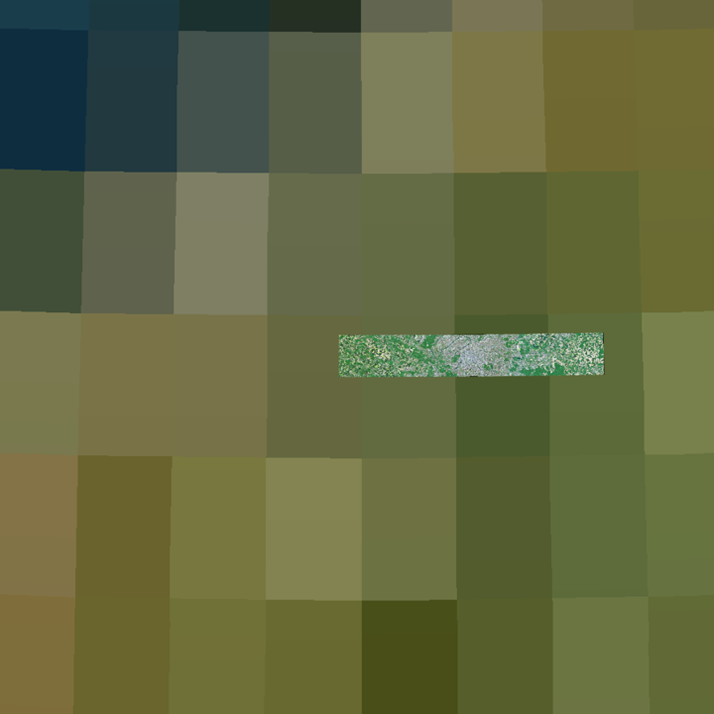
\includegraphics[width=0.4\linewidth]{figures/imageprocessing/HighResImage.png}
    \caption{This is the high resolution strip placed on the surface of the simulated Earth.}
    \label{fig:HighStrip}
\end{figure}

\noindent
To simulate the Earth's rotation, both the Earth and the high-resolution imagery patch are re-rendered at the rotational speed of the Earth, $\omega_e$
\vspace{0.5cm}

\noindent
To capture an image, the virtual camera is positioned at the satellite’s location within the simulator and oriented in a pure nadir direction. The resulting 
image is shown in Figure \ref{fig:GenSatImg}.

\begin{figure}[H]
    \centering
    \includegraphics[width=0.4\linewidth]{figures/imageprocessing/sat_image_001.png}
    \caption{An generated satellite imager as seen from the satellite imager}
    \label{fig:GenSatImg}
\end{figure}

%==========================================================================================================================================================
\mysubsection{Feature Detection}{Feature Detection}
\label{sec:FeatureDetection}

The images are first converted to grayscale and then processed using feature detection algorithms. MATLAB's feature detection functions allow the user 
to specify the number of feature points to detect. In Figure \ref{fig:FeatureDetection}, 20 of the strongest feature points were selected.
\vspace{0.5cm}

\noindent
SIFT is slower and more computationally intensive than SURF and ORB, but offers high accuracy, making it suitable for target recognition. SURF provides a faster alternative to SIFT, though with slightly reduced precision. ORB, using binary descriptors and Hamming distance for matching, is extremely fast and ideal for real-time applications, but is more sensitive to heavy noise and large scale variations. While ORB is widely used in real-time applications such as SLAM, it may struggle with rapidly changing satellite imagery, where a more robust approach such as SIFT or SURF would be more ideal. 

\begin{figure}[H]
    \centering
    \begin{subfigure}[b]{0.30\linewidth}
        \centering
        \includegraphics[width=\linewidth]{figures/imageprocessing/SIFT.png}
        \caption{Feature Dectection Using SIFT}
        \label{fig:SIFT}
    \end{subfigure}
    \hfill
    \begin{subfigure}[b]{0.30\linewidth}
        \centering
        \includegraphics[width=\linewidth]{figures/imageprocessing/SURF.png}
        \caption{Feature Detection Using SURF}
        \label{fig:SURF}
    \end{subfigure}
    \hfill
    \begin{subfigure}[b]{0.30\linewidth}
        \centering
        \includegraphics[width=\linewidth]{figures/imageprocessing/ORB.png}
        \caption{Feature Detection Using ORB}
        \label{fig:ORB}
    \end{subfigure}
    \caption{The french country side is used to compare the different feature points detected by SIFT, SURF and ORB}
    \label{fig:FeatureDetection}
\end{figure}

%============================================================================================================================================================
\mysubsection{Earth Tracker Algorithm}{Earth Tracker Algorithm}

\noindent
When a feature point is extracted from an image, it must be converted back into a feature vector, a process known as back-projection \cite{Korf}. This 
algorithm essentially performs the inverse of the camera model equation described in Section 4.3,

\begin{equation}
    \mathbf{f}_\mathcal{B}^+ = \mathbf{T}_\mathcal{C}^\mathcal{B} \times \mathbf{T}_\mathcal{M}^\mathcal{C} \times \mathbf{T}_\mathcal{P}^\mathcal{M} \times \mathbf{f}_\mathcal{P}^+ \text{.}
\end{equation}

\noindent
Where the transformation matrixes are defined as:

\begin{equation}
    \mathbf{T}_\mathcal{P}^\mathcal{M} = 
    \begin{bmatrix}
        \frac{1}{s_x}   & \alpha            & 0         & \frac{-c_x}{s_x} \\
        0               & \frac{1}{-s_y}    & 0         & \frac{-c_y}{-s_y} \\
        0               & 0                 & 1         & 0 \\
        0               & 0                 & 0         & 1        
    \end{bmatrix}
    \text{,}    
\end{equation}

\begin{equation}
    \mathbf{T}_\mathcal{M}^\mathcal{C} =
    \begin{bmatrix}
        \frac{-s}{f}I_{3\times3} & \boldsymbol{0}_{3\times1}\\
        \boldsymbol{0}_{1\times3} & 0
    \end{bmatrix}
    \text{, and}
\end{equation}

\begin{equation}
    \mathbf{T}_\mathcal{C}^\mathcal{B} = 
    \begin{bmatrix}
        (\mathbf{A}_\mathcal{B}^\mathcal{C})^T & \boldsymbol{0}_{3\times1} \\
         \boldsymbol{0}_{1\times3} & 1
    \end{bmatrix}
    \text{.}
\end{equation}


\noindent
All of these matrices are derived from the camera matrices defined in the camera model. This algorithm performs the 2D-to-3D projection, effectively reversing the 
3D-to-2D mapping of the camera. First, it converts a pixel point into coordinates on the camera's image plane in meters by translating the origin and applying the 
appropriate scaling factors, $s_x$ and $s_y$. The resulting values are then scaled to represent the feature as projected outside the satellite body frame.
\vspace{0.5cm}

\noindent
The scaling factor $s$ is particularly important, as information is inevitably lost during the 3D-to-2D projection. To resolve this ambiguity, an assumption about 
the satellite's operating altitude is required. Here, we assume an altitude of 500~km, giving a scaling factor of $s = 500~\text{km}$.

\begin{figure}[H]
    \centering
    \includegraphics[width=\linewidth]{figures/imageprocessing/ProjectionImage.png}
    \caption{An illustration of feature points being projected back to feature vectors.}
    \label{fig:ProjectionPoints}
\end{figure}

\noindent
In Figure \ref{fig:ProjectionPoints} the z-axis is scaled to show the feature vectors created by the Earth Tracker algorithm.
%=============================================================================================================================================================
\mysubsection{Catalogue Generation}{Catalogue Generation}
\label{sec:CatalogueGeneration}

In this work, creating a catalogue requires proper geolocation. Although feature matching is beyond the scope of this work and the features are randomly 
generated, the true position of the satellite is assumed, and raycasting is implemented to bypass feature matching.
\vspace{0.5cm}

\noindent
First the feature pixels are converted back to rays, exactly the same as the Earth Tracker, but is converted all the way to the ECI refrence frame.

\begin{equation}
        \mathbf{f}_\mathcal{I}^+ = \mathbf{T}_\mathcal{O}^\mathcal{I} \times \mathbf{T}_\mathcal{B}^\mathcal{O} \times \mathbf{T}_\mathcal{C}^\mathcal{B} \times \mathbf{T}_\mathcal{M}^\mathcal{C} \times 
        \mathbf{T}_\mathcal{P}^\mathcal{M} \times \mathbf{f}_\mathcal{P}^+ \text{.} \\
\end{equation}

\noindent
Then the vector is normalized

\begin{equation}
    \bar{\mathbf{f}}_\mathcal{I} =  \frac{\mathbf{f}_\mathcal{I}}{||\mathbf{f}_\mathcal{I}||} \text{.}
\end{equation}

\noindent
The intersection of a ray with the Earth ellipsoid is computed as follows. Let the ray in ECI coordinates be $\mathbf{p}(t) = \mathbf{r}_\mathcal{I} + t \, \bar{\mathbf{f}}_\mathcal{I}$, 
where $\mathbf{r}_\mathcal{I} = [x_0, y_0, z_0]^T$ is the satellite position and $\bar{\mathbf{f}}_\mathcal{I} = [dx, dy, dz]^T$ is the ray direction. 
Assuming the Earth is an ellipsoid with semi-major axis $a$ and semi-minor axis $b$, the quadratic equation for the intersection is

\begin{equation}
    A t^2 + B t + C = 0,
\end{equation}

\noindent
with coefficients
\begin{align*}
    A &= \frac{dx^2 + dy^2}{a^2} + \frac{dz^2}{b^2}, \\
    B &= 2 \left( \frac{x_0 dx + y_0 dy}{a^2} + \frac{z_0 dz}{b^2} \right), \text{and} \\
    C &= \frac{x_0^2 + y_0^2}{a^2} + \frac{z_0^2}{b^2} - 1.
\end{align*}

\noindent
The discriminant $\Delta = B^2 - 4AC$ determines whether the ray intersects the ellipsoid. If $\Delta < 0$, no intersection occurs. Otherwise, the solutions are

\begin{equation}
    t_1 = \frac{-B - \sqrt{\Delta}}{2A}, \quad
    t_2 = \frac{-B + \sqrt{\Delta}}{2A}.
\end{equation}

\noindent
The smallest positive root is chosen as $t_\text{intersect}$, corresponding to the closest intersection point in the direction of the ray. 
The intersection point in ECI coordinates is then
\begin{equation}
    \mathbf{p}_\mathcal{I} = \mathbf{r}_\mathcal{I} + t_\text{intersect} \, \bar{\mathbf{f}}_\mathcal{I}.
\end{equation}

\noindent
After that the feature ray is converted to the ECEF reference frame and then to the LLA point $\mathbf{p}_{LLA}$.

\begin{equation}
    \mathbf{p}_\text{LLA} = f(\mathbf{T}_\mathcal{I}^\mathcal{R} \times \mathbf{p}_\mathcal{I},\text{WGS84})
\end{equation}

\noindent
The Figure \ref{fig:GL} illustrates the end results  of this algorithm, which used to calculate the geolocations of the feature pixels to create the catalogue.

\begin{figure}[H]
    \centering
    \begin{subfigure}[b]{0.45\linewidth}
        \centering
        \includegraphics[width=\linewidth]{figures/imageprocessing/featurePixels.pdf}
        \caption{Satellite image with pixel locations of features detected.}
        \label{fig:PL}
    \end{subfigure}
    \hfill
    \begin{subfigure}[b]{0.48\linewidth}
        \centering
        \includegraphics[width=\linewidth]{figures/imageprocessing/GeoLocations.pdf}
        \caption{Satellite image of feature pixel locations geolocated using raycasting.}
        \label{fig:RC}
    \end{subfigure}
    \caption{Catalogue generation using raycasting.}
    \label{fig:GL}
\end{figure}

%========================
%==============================================================================================================================================================
\mysection{Conclusion}{Conclusion}

In this chapter, the process of converting visual odometry from a satellite image to Earth Tracker measurements is described. Firstly, the satellite
image geometry is discussed, including parameters such as the GSD, pitch, swath, and FOV. The different types of resolution obtainable from satellite imagery
are then explained, namely spatial, temporal, and radiometric resolution. The various methods of capturing these images are described, ranging from 
classical techniques such as pushbroom and whiskbroom sensors to more modern snapshot sensors. Each of these imagers must also contend with environmental noise sources such as clouds, 
atmospheric effects, and variations due to time of day or year.\\

\noindent
After the geometry of the image is explained, the camera itself is modeled using the pinhole model. From this, an unconventional intrinsic and 
extrinsic camera model, $\mathbf{T}_\mathcal{C}^\mathbf{P}$ and $\mathbf{T}_\mathcal{B}^\mathbf{C}$ respectively, is derived to mirror the format established 
in Chapter 3. Following the camera modeling, the lens is also modeled. While many types of lens distortions exist, this work focuses on two geometric distortions 
(radial and tangential) and one radiometric distortion (chromatic aberration).\\

\noindent
Finally, the Earth Tracker itself is addressed. The image generation process is first described by adding a high-resolution patch to the 
simulator for the Earth Tracker to use. The Earth Tracker algorithm is then derived from the intrinsic and extrinsic camera parameters and uses back projection to convert
from a 2D feature point to a 3D feature vector. For proper pose estimation the feature geolocation is also needed, but to bypass the feature matching process raycasting is described
and used.




%==============================================================================================================================================================